
\begin{frame}{}
    \begin{center}
        \large \textbf{Transformer-XL (extra-large)}
    \end{center}
    \vspace{20pt}
    
    \textbf{Author(s):}
    \begin{itemizeSpaced}{5pt}
    {\color{DimGrey} 
    
        \item Dai et al. (2019) in \emph{Transformer-XL: Attentive Language Models Beyond a Fixed-Length Context}
        
    }
    \end{itemizeSpaced}
\end{frame}

% -------------------------------------------------



\begin{frame}{Problem with Transformer}
    
    \begin{alertBlock}{Warning: Fixed-Length Context}
        \footnotesize 
        
        Transformers have \textbf{\alert{fixed-length context}} (context dependency limited by input length) \newline 
        
        Natural semantic boundaries formed by sentences are \textit{not} respected.\newline  
        
        \begin{addmargin}{3em}{}
        \begin{itemizeSpaced}{2pt}
            \footnotesize 
            
            \arrowitem Transformers lose context
            
            \arrowitem Transformers forget words from a few sentences ago 
            
            \arrowitem \textbf{Context-Fragmentation Problem}
        \end{itemizeSpaced}
        \end{addmargin} 
        
    \end{alertBlock}
    

\end{frame}
    
    
\begin{frame}{Problem with Transformer: Fixed-Length Context Illustrated}
    

    \begin{figure}[h]
    \vspace{-5pt}
    \centering
    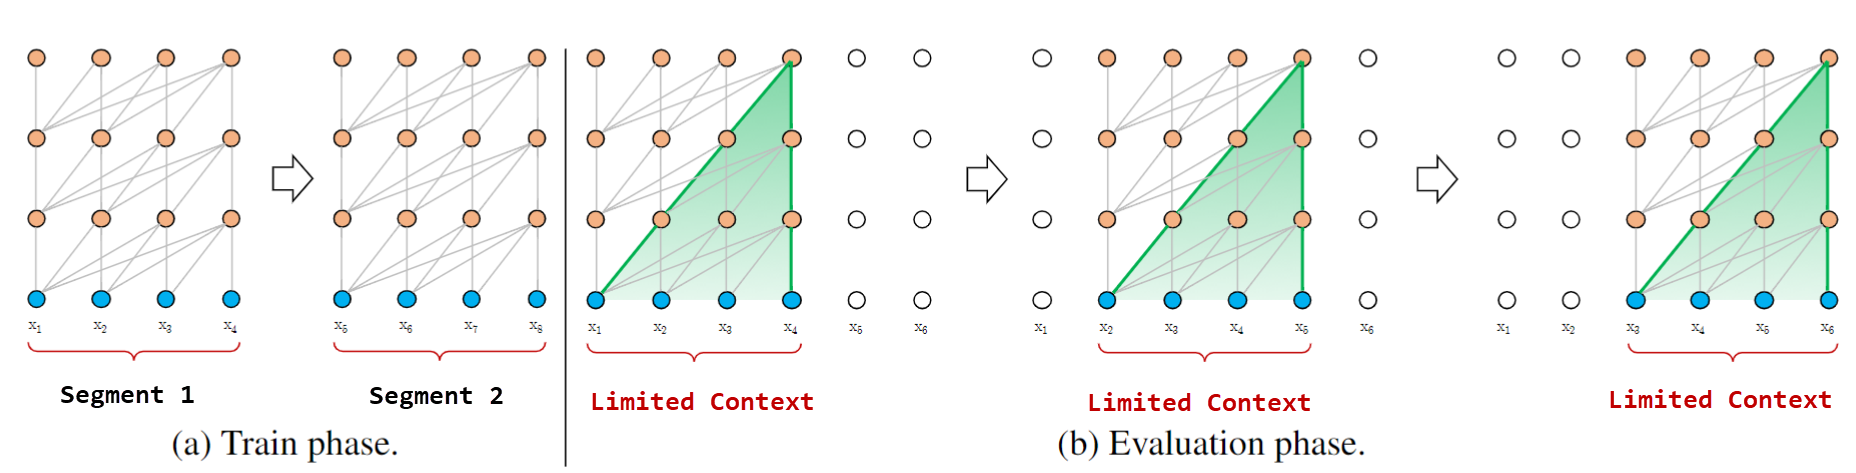
\includegraphics[width=0.99\textwidth]{imgs/transXL_vanillaSegmentation.png}
    %\vspace{-5pt}
    \caption{Vanilla Transformer with segment embedding length $ = 4$. Training the model in fixed-length segments while disregarding natural sentence boundaries results in the \emph{context fragmentation problem}: during each evaluation step, the Transformer consumes a segment embedding and makes a prediction at the last position. Then {\color{Teal} at the next step, the segment is shifted right by one position only, and the new segment must be processed from scratch, so there is limited context dependency ... between segments.} From \emph{Transformer-XL: Attentive Language Models Beyond a Fixed-Length Context}, by Dai et al., 2019. \url{https://arxiv.org/pdf/1901.02860.pdf}. Copyright 2019 by Dai et al.}
    \vspace{-5pt}
    \label{fig:transXL_VanillaSegment}
    \end{figure}
    
\end{frame}



\begin{frame}{\large Motivation for Transformer-XL}

    \begin{itemizeSpaced}{15pt}
    \small 
    
        \item \textbf{Transformer-XL} (extra long) learns longer dependencies without ``disrupting temporal coherence"  (Dai et al., 2019). 
        
        \item Doesn't chop sentences into arbitrary \textbf{fixed lengths}!
        
        \pinkbox Transformer-XL \emph{respects natural language boundaries} like sentences and paragraphs, helping it gain richer context for these and longer texts like documents. 
        
       % \pinkbox Transformer-XL is composed of \textbf{segment-level recurrence mechanism} and \textbf{relative positional encoding} method (to fix \textbf{context fragmentation} and represent longer-spanning dependencies)
    \end{itemizeSpaced}
    
\end{frame}


\begin{frame}{Transformer-XL: Segment-Level Recurrence Mechanism}

    \vspace{20pt}
    
    When a segment is being processed, each hidden layer receives two inputs: 
    
    \begin{itemizeSpaced}{5pt}
        \item the previous hidden layer outputs of the \emph{current segment} (like vanilla transformer, visible as gray arrows in \cref{fig:transXL_extendedContext})
        
        \item the previous hidden layer outputs of the \emph{previous segment} (green arrows in \cref{fig:transXL_extendedContext}).
    \end{itemizeSpaced}
    
    
    
    \begin{figure}[h]
    \vspace{-5pt}
    \centering
    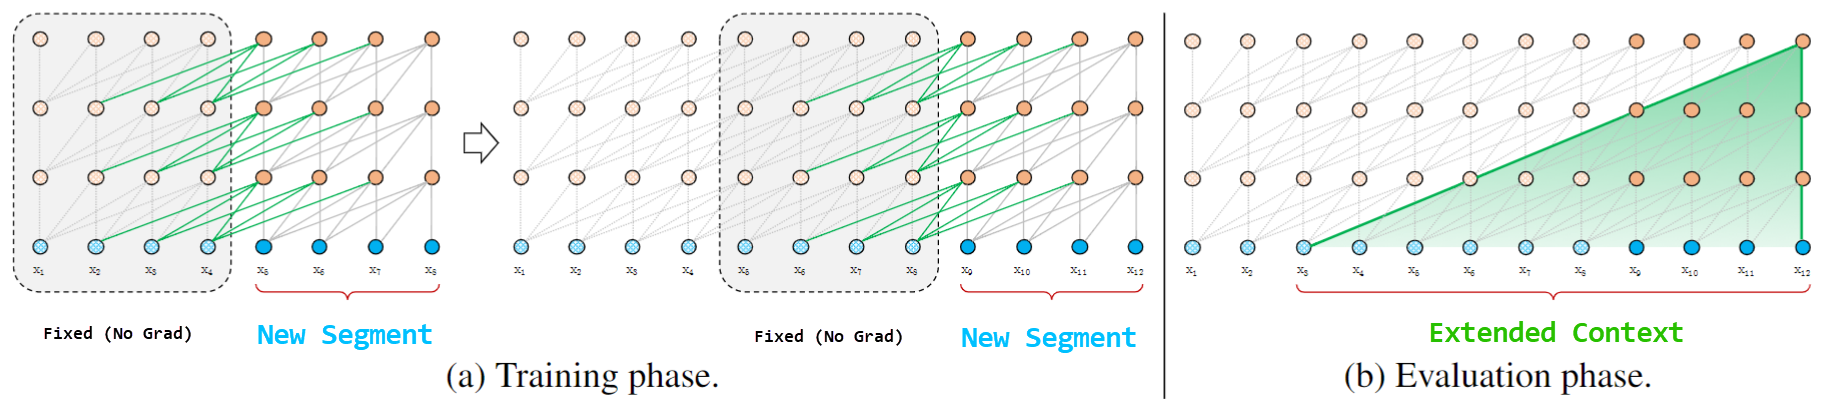
\includegraphics[width=0.99\textwidth]{imgs/transXL_extendedcontext.png}
    %\vspace{-5pt}
    \caption{ Segment level recurrence mechanism at work: the hidden state for previous segment is \emph{fixed} and \emph{stored} to later be reused as extended context while new segment is processed. Like in Transformer, gradient updates (training) still occurs within a segment, but extended context includes historical information. From \emph{Transformer-XL: Attentive Language Models Beyond a Fixed-Length Context}, by Dai et al., 2019. \url{https://arxiv.org/pdf/1901.02860.pdf}. Copyright 2019 by Dai et al.}
    %\vspace{-5pt}
    \label{fig:transXL_extendedContext}
    \end{figure}
    
\end{frame}


% ERASE - not important
% \begin{frame}{Transformer-XL: Relative Positional Encoding}
%     \vspace{20pt}
%     
%     \begin{alertBlock}{Problem when using Segment-Level Recurrence}
%         \footnotesize 
%         How can we keep \alert{word order when reusing hidden states?}\newline 
%         
%         When applying standard positional encodings to Transformer-XL...\newline 
%         
%         \begin{addmargin}{3em}{} % 3em left, NOTHING right
%         \begin{itemizeSpaced}{5pt}
%             
%             \largearrowitem Tokens from different segments got SAME positional encodings
%             
%             \largearrowitem Transformer-XL couldn't distinguish positions of consecutive inputs.
%             
%             \largearrowitem Ruined the point of positional encodings!
%             
%         \end{itemizeSpaced}
%         \end{addmargin} 
%         
%         
%     \end{alertBlock} 
%     
%     
%     \vspace{7pt}
%     
%     {\footnotesize \textbf{The Solution ... }}
%     
%     \vspace{7pt}
%     
%     \begin{addmargin}{3em}{}
%     \begin{itemizeSpaced}{0pt}
%         \largearrowitem {\color{ForestGreen} \textbf{Relative Positional Encodings}} to encode \emph{relative} distance between tokens not their \emph{absolute} distance. 
%     \end{itemizeSpaced}
%     \end{addmargin}
% 
%     
% \end{frame}


% 
% \begin{frame}{Transformer-XL: Experimental Results}
%     
%     \vspace{20pt}
%     
%     \textbf{Ablation study:} Isolating effects of \textbf{segment-level recurrence mechanism} with different encoding schemes (Shaw (2018) uses relative, and Vaswani / Al-Rfou use absolute).
%         
%     \vspace{-10pt}
%     \begin{figure}[h]
%     \vspace{-5pt}
%     \centering
%     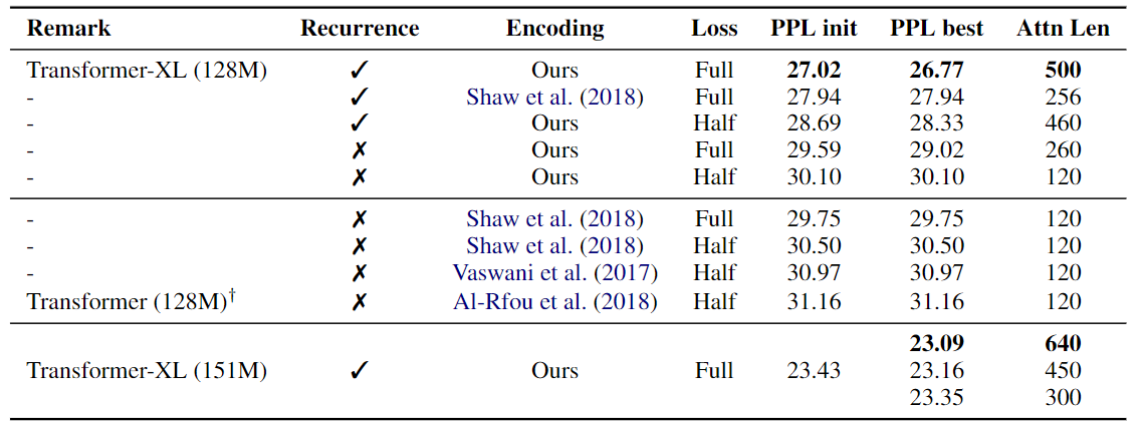
\includegraphics[width=0.99\textwidth]{imgs/table_transXL_ablationREC.png}
%     \vspace{-5pt}
%     \captionof{table}{\linespread{0.1} \textbf{PPL best} (model output) means perplexity score obtained using an optimal backpropagation training time length. \textbf{Attn Len} (model input) is the shortest possible attention length during evaluation to achieve the corresponding PPL best. From \emph{Transformer-XL: Attentive Language Models Beyond a Fixed-Length Context}, by Dai et al., 2019. \url{https://arxiv.org/pdf/1901.02860.pdf}. Copyright 2019 by Dai et al.}
%     \vspace{-5pt}
%     \label{tbl:transXL_ablationRECURR}
%     \end{figure}
% 
% \end{frame}